\section{Parallel Design}

In this section, we analyze the design space for parallelizing the Cholesky
factorization. We explore different strategies for data distribution and
processor organization, highlighting the limitations of naive approaches and
justifying our final choice.

\subsection{Evaluation of Intermediate Strategies}
The core challenge is mapping the matrix onto the processors efficiently. We
considered some evolutionary steps to identify the optimal strategy.

\subsubsection{Step 1: 1D Row Decomposition (The Naive Approach)}
The simplest strategy is to slice the matrix horizontally. We assign contiguous
groups of rows to each processor. For example, Processor 1 gets the first row,
Processor 1 gets the second row...

\textbf{Visualization:}
If we strictly assign one row per processor:

\begin{figure}[h]
    \centering
    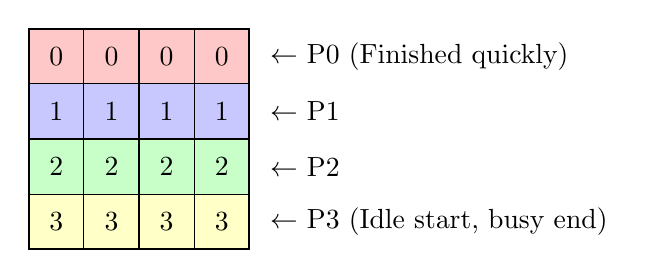
\begin{tikzpicture}[scale=0.7]
        % Define colors
        \definecolor{p0}{RGB}{255, 200, 200}
        \definecolor{p1}{RGB}{200, 200, 255}
        \definecolor{p2}{RGB}{200, 255, 200}
        \definecolor{p3}{RGB}{255, 255, 200}

        % --- ROW 0 (Processor 0) ---
        \fill[p0] (0,3) rectangle (4,4);
        % Place numbers individually
        \foreach \x in {0.5, 1.5, 2.5, 3.5} \node at (\x, 3.5) {0};
        \node[anchor=west] at (4.2, 3.5) {$\leftarrow$ P0 (Finished quickly)};

        % --- ROW 1 (Processor 1) ---
        \fill[p1] (0,2) rectangle (4,3);
        \foreach \x in {0.5, 1.5, 2.5, 3.5} \node at (\x, 2.5) {1};
        \node[anchor=west] at (4.2, 2.5) {$\leftarrow$ P1};

        % --- ROW 2 (Processor 2) ---
        \fill[p2] (0,1) rectangle (4,2);
        \foreach \x in {0.5, 1.5, 2.5, 3.5} \node at (\x, 1.5) {2};
        \node[anchor=west] at (4.2, 1.5) {$\leftarrow$ P2};

        % --- ROW 3 (Processor 3) ---
        \fill[p3] (0,0) rectangle (4,1);
        \foreach \x in {0.5, 1.5, 2.5, 3.5} \node at (\x, 0.5) {3};
        \node[anchor=west] at (4.2, 0.5) {$\leftarrow$ P3 (Idle start, busy end)};

        % Grid and Border
        \draw[step=1cm, black, thin] (0,0) grid (4,4);
        \draw[black, thick] (0,0) rectangle (4,4);
    \end{tikzpicture}
    \caption{Visualization of 1D Row Decomposition.}
    \label{fig:1d_row_decomp}
\end{figure}

\begin{itemize}
    \item \textbf{Limitation:} As the algorithm moves down the diagonal (from
        row 0 to 3), the top processors finish their work and become idle.
        Processor 0 does nothing after the first step. This leads to
        \textbf{poor load balancing}.
\end{itemize}

\subsubsection{Step 2: 1D Cyclic Decomposition}
To solve the load balancing issue, we can distribute rows in a round-robin
fashion (like dealing cards). 

\begin{figure}[h]
    \centering
    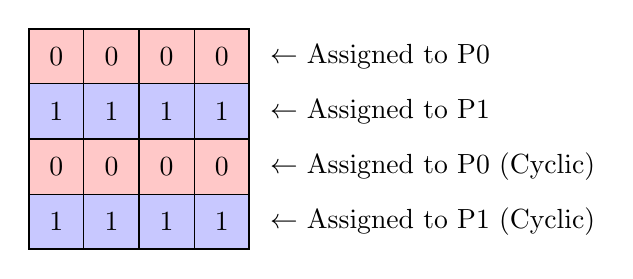
\begin{tikzpicture}[scale=0.7]
        % Define colors
        \definecolor{p0}{RGB}{255, 200, 200}
        \definecolor{p1}{RGB}{200, 200, 255}

        % --- ROW 0 (Processor 0) ---
        \fill[p0] (0,3) rectangle (4,4);
        \foreach \x in {0.5, 1.5, 2.5, 3.5} \node at (\x, 3.5) {0};
        \node[anchor=west] at (4.2, 3.5) {$\leftarrow$ Assigned to P0};

        % --- ROW 1 (Processor 1) ---
        \fill[p1] (0,2) rectangle (4,3);
        \foreach \x in {0.5, 1.5, 2.5, 3.5} \node at (\x, 2.5) {1};
        \node[anchor=west] at (4.2, 2.5) {$\leftarrow$ Assigned to P1};

        % --- ROW 2 (Processor 0 AGAIN) ---
        \fill[p0] (0,1) rectangle (4,2);
        \foreach \x in {0.5, 1.5, 2.5, 3.5} \node at (\x, 1.5) {0};
        \node[anchor=west] at (4.2, 1.5) {$\leftarrow$ Assigned to P0 (Cyclic)};

        % --- ROW 3 (Processor 1 AGAIN) ---
        \fill[p1] (0,0) rectangle (4,1);
        \foreach \x in {0.5, 1.5, 2.5, 3.5} \node at (\x, 0.5) {1};
        \node[anchor=west] at (4.2, 0.5) {$\leftarrow$ Assigned to P1 (Cyclic)};

        % Grid and Border
        \draw[step=1cm, black, thin] (0,0) grid (4,4);
        \draw[black, thick] (0,0) rectangle (4,4);

    \end{tikzpicture}
    \caption{Visualization of 1D Cyclic Decomposition.}
    \label{fig:1d_cyclic_decomp}
\end{figure}

\begin{itemize}
    \item \textbf{Limitation:} While computation is balanced,
        \textbf{communication is inefficient}. After factorizing a diagonal
        block, the owner must broadcast the result so that other processors
        can update the column elements below it. Since the rows are
        distributed cyclically among \textit{all} $P$ processors, almost
        every processor owns a part of that column. Consequently, the
        broadcast becomes a global operation involving the entire cluster.
        This wastes network bandwidth because it forces a global
        synchronization, whereas a more optimized design would restrict
        this traffic to only a small vertical subset of processors.
\end{itemize}

\subsubsection{Step 3: Introduction of Block Algorithms}
Before optimizing communication, we address the computational efficiency of the
node.

\textbf{The Problem (Memory Hierarchy):}
Accessing data from the main memory (RAM) is significantly slower than
performing calculations in the CPU. If the algorithm processes single elements
one by one, the processor frequently waits for data to arrive from RAM.

\textbf{The Solution (Blocking):}
To mitigate this latency, we divide the matrix into square sub-matrices called
\textbf{blocks} (e.g., $64 \times 64$). When a block is accessed, it can remain
in the CPU’s cache across multiple operations. Since the Cholesky algorithm
performs many operations on the same data, working on blocks allows the
processor to reuse the data residing in the Cache multiple times before needing
to access the RAM again.

\begin{figure}[h]
    \centering
    \begin{tabular}{c c}
        % Left side: Standard Element-wise
        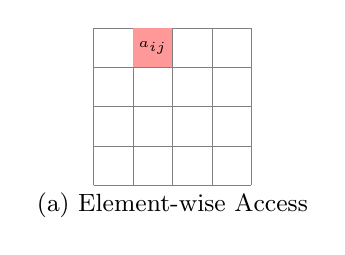
\begin{tikzpicture}[scale=0.5]
            \draw[step=1cm,gray,very thin] (0,0) grid (4,4);
            \node at (2, -0.5) {\small (a) Element-wise Access};
            % Highlight one tiny cell
            \fill[red!40] (1,3) rectangle (2,4);
            \node at (1.5, 3.5) {\tiny $a_{ij}$};
        \end{tikzpicture}
&
% Right side: Block-wise
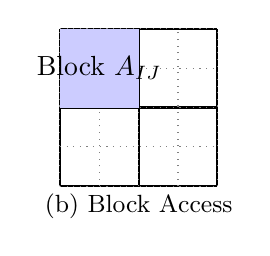
\begin{tikzpicture}[scale=0.5]
    \draw[step=2cm,black,thick] (0,0) grid (4,4);
    \draw[step=1cm,gray,dotted] (0,0) grid (4,4);
    \node at (2, -0.5) {\small (b) Block Access};
    % Highlight one big block
    \fill[blue!20] (0,2) rectangle (2,4);
    \node at (1, 3) {Block $A_{IJ}$};
\end{tikzpicture}
    \end{tabular}
    \caption{Comparison between (a) accessing single elements vs (b) loading a full block.}
    \label{fig:blocking_schema}
\end{figure}

\begin{itemize}
    \item \textbf{Impact:} This improves the ratio of computation to memory
        access, resulting in higher computational throughput, measured in
        GFLOPS (Giga Floating Point Operations Per Second), compared to the
        element-wise approach.
\end{itemize}


\subsection{Proposed Solution: 2D Block-Cyclic Decomposition}
By combining the strengths of the previous steps (Load Balancing + Blocking),
we implemented the \textbf{2D Block-Cyclic Decomposition}. This is the optimal
strategy because it solves the communication bottleneck of Step 2 by arranging
processors in a grid.

\subsubsection{Process Grid and Distribution Logic}
To implement the 2D decomposition, we first organize the available processors
into a logical grid. For example, if we have $P = 4$ processors, we arrange
them into a $2 \times 2$ grid ($R=2, C=2$).

Each processor is identified by its coordinates $(P_{row}, P_{col})$:
\[
    \begin{matrix}
        (0,0) & (0,1) \\
        (1,0) & (1,1)
    \end{matrix}
    \quad \longrightarrow \quad
    \begin{matrix}
        P_0 & P_1 \\
        P_2 & P_3
    \end{matrix}
\]

\textbf{Mapping Blocks:}
We do not distribute single elements. We view the global matrix $A$ as a grid
of blocks, where each block contains $B \times B$ elements (e.g., $64
\times 64$). We map these blocks to processors in a round-robin (cyclic)
fashion.

The owner of a block at global block index $(i, j)$ is determined by:
\begin{equation}
    \begin{aligned}
        P_{row} &= i \pmod R \\
        P_{col} &= j \pmod C
    \end{aligned}
\end{equation}

\begin{figure}[h]
    \centering
    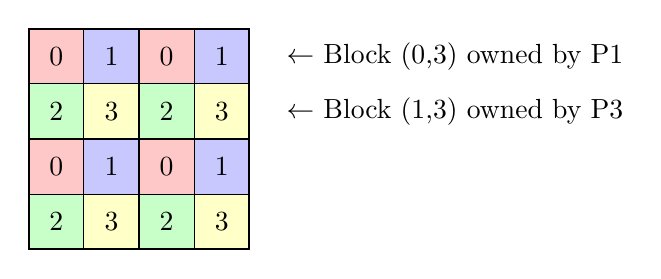
\begin{tikzpicture}[scale=0.7]
        % Define colors
        \definecolor{p0}{RGB}{255, 200, 200}
        \definecolor{p1}{RGB}{200, 200, 255}
        \definecolor{p2}{RGB}{200, 255, 200}
        \definecolor{p3}{RGB}{255, 255, 200}

        % --- ROW 0 ---
        \fill[p0] (0,3) rectangle (1,4); \node at (0.5, 3.5) {0};
        \fill[p1] (1,3) rectangle (2,4); \node at (1.5, 3.5) {1};
        \fill[p0] (2,3) rectangle (3,4); \node at (2.5, 3.5) {0};
        \fill[p1] (3,3) rectangle (4,4); \node at (3.5, 3.5) {1};

        % --- ROW 1 ---
        \fill[p2] (0,2) rectangle (1,3); \node at (0.5, 2.5) {2};
        \fill[p3] (1,2) rectangle (2,3); \node at (1.5, 2.5) {3};
        \fill[p2] (2,2) rectangle (3,3); \node at (2.5, 2.5) {2};
        \fill[p3] (3,2) rectangle (4,3); \node at (3.5, 2.5) {3};

        % --- ROW 2 ---
        \fill[p0] (0,1) rectangle (1,2); \node at (0.5, 1.5) {0};
        \fill[p1] (1,1) rectangle (2,2); \node at (1.5, 1.5) {1};
        \fill[p0] (2,1) rectangle (3,2); \node at (2.5, 1.5) {0};
        \fill[p1] (3,1) rectangle (4,2); \node at (3.5, 1.5) {1};

        % --- ROW 3 ---
        \fill[p2] (0,0) rectangle (1,1); \node at (0.5, 0.5) {2};
        \fill[p3] (1,0) rectangle (2,1); \node at (1.5, 0.5) {3};
        \fill[p2] (2,0) rectangle (3,1); \node at (2.5, 0.5) {2};
        \fill[p3] (3,0) rectangle (4,1); \node at (3.5, 0.5) {3};

        % Grid and Border
        \draw[step=1cm, black, thin] (0,0) grid (4,4);
        \draw[black, thick] (0,0) rectangle (4,4);

        % Small Note
        \node[anchor=west] at (4.5, 3.5) {$\leftarrow$ Block (0,3) owned by P1};
        \node[anchor=west] at (4.5, 2.5) {$\leftarrow$ Block (1,3) owned by P3};
    \end{tikzpicture}
    \caption{Visualization of 2D Block-Cyclic distribution. Each square
        represents a \textbf{data block} (e.g., $64 \times 64$ doubles), not a
        single element.}
    \label{fig:2d_block_cyclic}
\end{figure}

\textbf{Why this mapping is effective:}
This distribution scatters the blocks owned by a single processor across the
entire matrix. As seen in Figure \ref{fig:2d_block_cyclic}, \textit{Processor 0}
owns blocks at grid positions $(0,0), (0,2), (2,0),$ and $(2,2)$. Even when the
"active" part of the matrix shrinks (e.g., after the first few iterations),
Processor 0 still holds valid blocks further down the matrix (at row 2),
ensuring it remains busy and contributing to the computation.

\textbf{Communication Efficiency:}
Beyond load balancing, this grid structure fundamentally changes the
communication pattern. In a 1D distribution (Step 2), a broadcast involves all
$P$ processors. In this 2D grid, operations like broadcasting a diagonal block
or a panel are restricted to the processors in a specific row or column
(involving only $\sqrt{P}$ processors). This reduces network contention and
significantly improves scalability as the cluster size grows.

\begin{figure}[h]
    \centering
    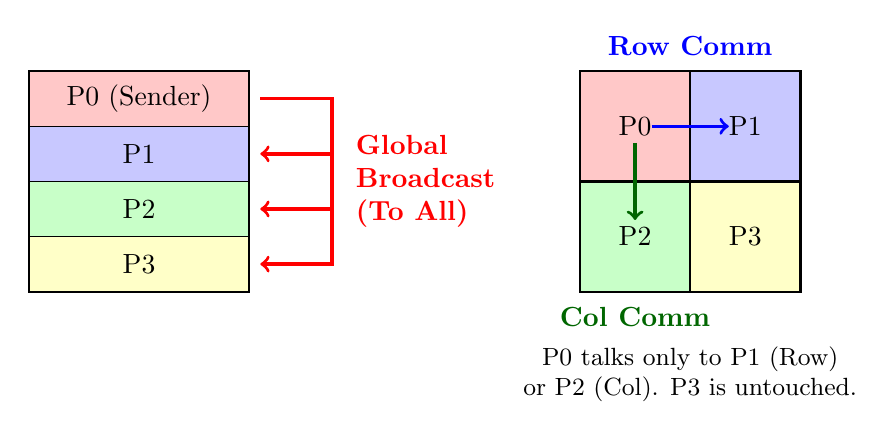
\begin{tikzpicture}[scale=0.7]
        % Define standard colors (Same as previous figures)
        \definecolor{p0}{RGB}{255, 200, 200} % Redish
        \definecolor{p1}{RGB}{200, 200, 255} % Blueish
        \definecolor{p2}{RGB}{200, 255, 200} % Greenish
        \definecolor{p3}{RGB}{255, 255, 200} % Yellowish

        % --- LEFT: 1D Global Broadcast ---
        % Stack processors vertically to represent 1D list
        \fill[p0] (0,3) rectangle (4,4); \node at (2,3.5) {P0 (Sender)};
        \fill[p1] (0,2) rectangle (4,3); \node at (2,2.5) {P1};
        \fill[p2] (0,1) rectangle (4,2); \node at (2,1.5) {P2};
        \fill[p3] (0,0) rectangle (4,1); \node at (2,0.5) {P3};

        % Draw borders
        \draw[thick] (0,0) rectangle (4,4);
        \draw (0,1) -- (4,1); \draw (0,2) -- (4,2); \draw (0,3) -- (4,3);

        % Arrows (Global Broadcast)
        \draw[->, very thick, red] (4.2, 3.5) -- (5.5, 3.5) -- (5.5, 2.5) -- (4.2, 2.5);
        \draw[->, very thick, red] (5.5, 2.5) -- (5.5, 1.5) -- (4.2, 1.5);
        \draw[->, very thick, red] (5.5, 1.5) -- (5.5, 0.5) -- (4.2, 0.5);

        % Label
        \node[red, align=left, font=\bfseries] at (7.2, 2) {Global\\Broadcast\\(To All)};

        % --- RIGHT: 2D Grid Broadcast ---
        \begin{scope}[xshift=10cm]
            % Draw 2x2 Grid with correct colors
            \fill[p0] (0,2) rectangle (2,4); \node at (1,3) {P0};
            \fill[p1] (2,2) rectangle (4,4); \node at (3,3) {P1};
            \fill[p2] (0,0) rectangle (2,2); \node at (1,1) {P2};
            \fill[p3] (2,0) rectangle (4,2); \node at (3,1) {P3};

            % Borders
            \draw[thick] (0,0) rectangle (4,4);
            \draw[thick] (2,0) -- (2,4);
            \draw[thick] (0,2) -- (4,2);

            % Row Comm Arrow
            \draw[->, very thick, blue] (1.3, 3) -- (2.7, 3);
            \node[blue, font=\bfseries, anchor=south] at (2, 4.1) {Row Comm};

            % Col Comm Arrow
            \draw[->, very thick, black!60!green] (1, 2.7) -- (1, 1.3);
            \node[black!60!green, font=\bfseries, anchor=north] at (1, -0.1) {Col Comm};

            % Label Explanation
            \node[align=center, font=\small] at (2, -1.5) {P0 talks only to P1 (Row)\\or P2 (Col). P3 is untouched.};
        \end{scope}
    \end{tikzpicture}
    \caption{Communication Pattern Comparison. Left: In 1D, P0 must send to everyone. Right: In 2D, communication is restricted to the specific Row or Column subset.}
    \label{fig:comm_pattern}
\end{figure}

\subsection{Parallel Algorithm Workflow}
With the data distributed across the 2D grid, the Cholesky factorization
proceeds in iterations $k=0 \dots N_{blocks}-1$. In each iteration, we process
one block column and update the rest of the matrix.

Since we are not using external linear algebra libraries, we implemented the
standard Level-3 BLAS operations manually.

\subsubsection{Phase 1: Factorize Diagonal Block (POTRF)}
The process that owns the current diagonal block ($P_{diag}$) computes the
Cholesky factorization of that single block locally.
\[ A_{kk} \leftarrow \text{Chol}(A_{kk}) \]
\begin{itemize}
    \item \textbf{Action:} We perform a sequential Cholesky factorization on
        the local $B \times B$ block to obtain the lower triangular factor
        $L_{kk}$.
    \item \textbf{Communication:} $P_{diag}$ broadcasts $L_{kk}$ vertically to
        all other processors in the same \textbf{grid column}.
\end{itemize}

\subsubsection{Phase 2: Update Panel (TRSM)}
All processors in the current process column must update their blocks $A_{ik}$
located below the diagonal. This corresponds to solving a triangular system of
equations:
\[ A_{ik} \leftarrow A_{ik} (L_{kk}^T)^{-1} \]
\begin{itemize}
    \item \textbf{Action:} We implemented the \textbf{TRSM} (Triangular Solve
        with Multiple Right-Hand Sides) algorithm. Since $L_{kk}^T$ is upper
        triangular, we solve the system $X L_{kk}^T = A_{ik}$ using forward
        substitution.
    \item \textbf{Communication:} Once updated, these blocks are broadcast
        horizontally to all processors in their respective \textbf{grid rows}.
\end{itemize}

\subsubsection{Phase 3: Update Trailing Matrix (GEMM / SYRK)}
Finally, all processors update their local portion of the remaining submatrix
using the data received from the broadcasts.
\[ A_{ij} \leftarrow A_{ij} - A_{ik} A_{jk}^T \]
\begin{itemize}
    \item \textbf{Action:} We implemented the update using a unified loop
        structure restricted to $j \le i$. This \textit{exploits the matrix
        symmetry} to reduce computational cost. By updating only the unique
        blocks in the lower triangle, we avoid redundant calculations for the
        upper triangular part (which is logically identical but not
        stored/accessed).
\end{itemize}


\subsection{Analysis of Parallelism and Dependencies}
To understand the scalability of our design, we must analyze the \textbf{data
dependencies} that dictate which operations can be performed in parallel and
which must be serialized.

\subsubsection{Data Dependencies}
The Cholesky algorithm has a strict dependency chain:
\begin{enumerate}
    \item \textbf{Diagonal Dependency:} The diagonal block $A_{kk}$ must be
        factorized first. No other operation in the current iteration $k$ can
        proceed until this is finished.
    \item \textbf{Panel Dependency:} The blocks in the current column $A_{ik}$
        cannot be updated until they receive the factorized diagonal block
        $L_{kk}$.
    \item \textbf{Trailing Matrix Dependency:} The update of any trailing block
        $A_{ij}$ (where $i,j > k$) requires the corresponding updated blocks
        from the current panel ($A_{ik}$ and $A_{jk}$).
\end{enumerate}

\subsubsection{The Opportunity for Parallelism}
Despite these dependencies, the algorithm exposes massive parallelism in the
\textit{Trailing Matrix Update (Phase 3)}. Once the panel broadcast is
complete, the update of each block $A_{ij}$ in the trailing submatrix is
\textit{mathematically independent} of all other block updates in that
submatrix. \[ A_{ij}^{(new)} = A_{ij}^{(old)} - A_{ik} \cdot A_{jk}^T \] This
independence allows every processor to update all its local blocks
simultaneously without synchronization with neighbors.

\subsubsection{Degree of Concurrency}
The available parallelism (concurrency) varies by phase:
\begin{itemize}
    \item \textbf{Phase 1 (Diagonal):} \textbf{Serial bottleneck.} Only 1
        process is active.
    \item \textbf{Phase 2 (Panel):} \textbf{Partial Parallelism.} Only
        $\sqrt{P}$ processes (one column) are active.
    \item \textbf{Phase 3 (Trailing):} \textbf{Full Parallelism.} All $P$
        processes are active.
\end{itemize}
Since Phase 3 dominates the computational cost (performing $O(N^3)$ operations
versus $O(N^2)$ for the panel), the highly parallel part hides the inefficiency
of the serial and partial phases as the matrix size $N$ grows.
